\subsection{Visual Representations of States and Actions}
%Conventionally, the space for rendering a state is limited because a small portion of the display area is reserved for provenance information; whereas, the much larger portion is used for data exploration \cite{Shrinivasan2008, Gotz2009, Kadivar2009}. Therefore, a small-scale visualization of the captured state is popular \cite{Hightower1998} (Figure \ref{fig:lr-state-1}). To recall the affect of the performed action, the miniature can highlight the difference from the previous state \cite{Klemmer2002} (Figure \ref{fig:lr-state-2}), or combine both the former and the latter visualizations corresponding to that action \cite{Kurlander1988} (Figure \ref{fig:lr-state-3}).

\subsubsection{State}
\begin{itemize}
	\item snapshot of the interface
	\item improved by highlighting changes (todo: read ~\cite{Waterson2002})
\end{itemize}

\begin{figure}[!htb]
\centering
\subcaptionbox{A snapshot of a web page. \emph{Image source:~\cite{Hightower1998}}\label{fig:lr-state-1}.}{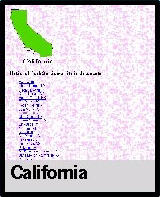
\includegraphics[height=.33\columnwidth]{state-1}} 
\hfill
\subcaptionbox{Modified post-it notes are highlighted with green borders. \emph{Image source:~\cite{Klemmer2002}}.\label{fig:lr-state-2}}{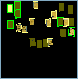
\includegraphics[height=.33\columnwidth]{state-2}} 
\hfill
\subcaptionbox{A graphical editor shows two states: before and after the last action. \emph{Image source:~\cite{Kurlander1988}}.\label{fig:lr-state-3}}[.34\columnwidth]{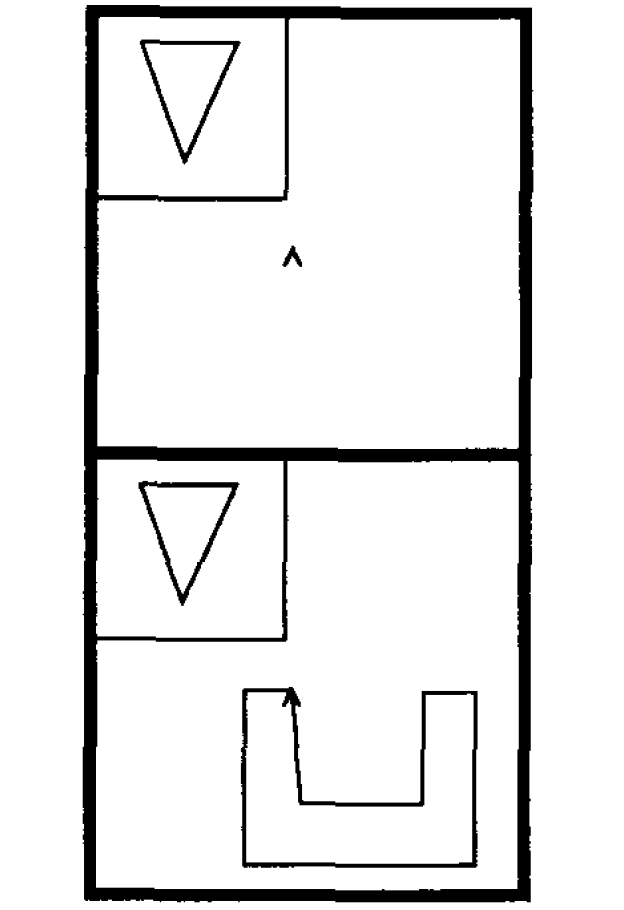
\includegraphics[height=.33\columnwidth]{state-3}}
\caption{Visual representations of states.}
\end{figure}

\subsubsection{Action}
%Typically, a system supports a certain number of actions; and thus allows using icons to visually distinguish different kinds of actions besides texts \cite{Gotz2009} (Figure \ref{fig:lr-action-1}). Actions are also commonly represented as edges in a graph to connect two states. Therefore, graph edges can be stylised to reflect the characteristics of the represented actions \cite{Ma1999} (Figure \ref{fig:lr-action-2}).

\begin{itemize}
	\item text such as in History menu of web browser
	\item improved by highlighting changes (todo: read ~\cite{Waterson2002})
\end{itemize}

\begin{figure}[!htb]
\centering
\subcaptionbox{Icon. \emph{Image source:~\cite{Gotz2009}}.\label{fig:lr-action-1}}{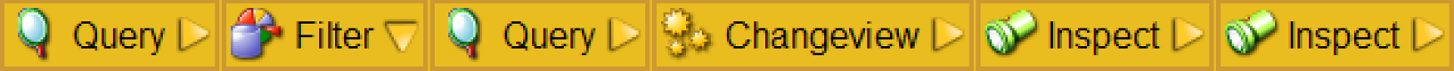
\includegraphics[width=.7\columnwidth]{action-1}}
\subcaptionbox{Stylish edges. \emph{Image source:~\cite{Ma1999}}.\label{fig:lr-action-2}}{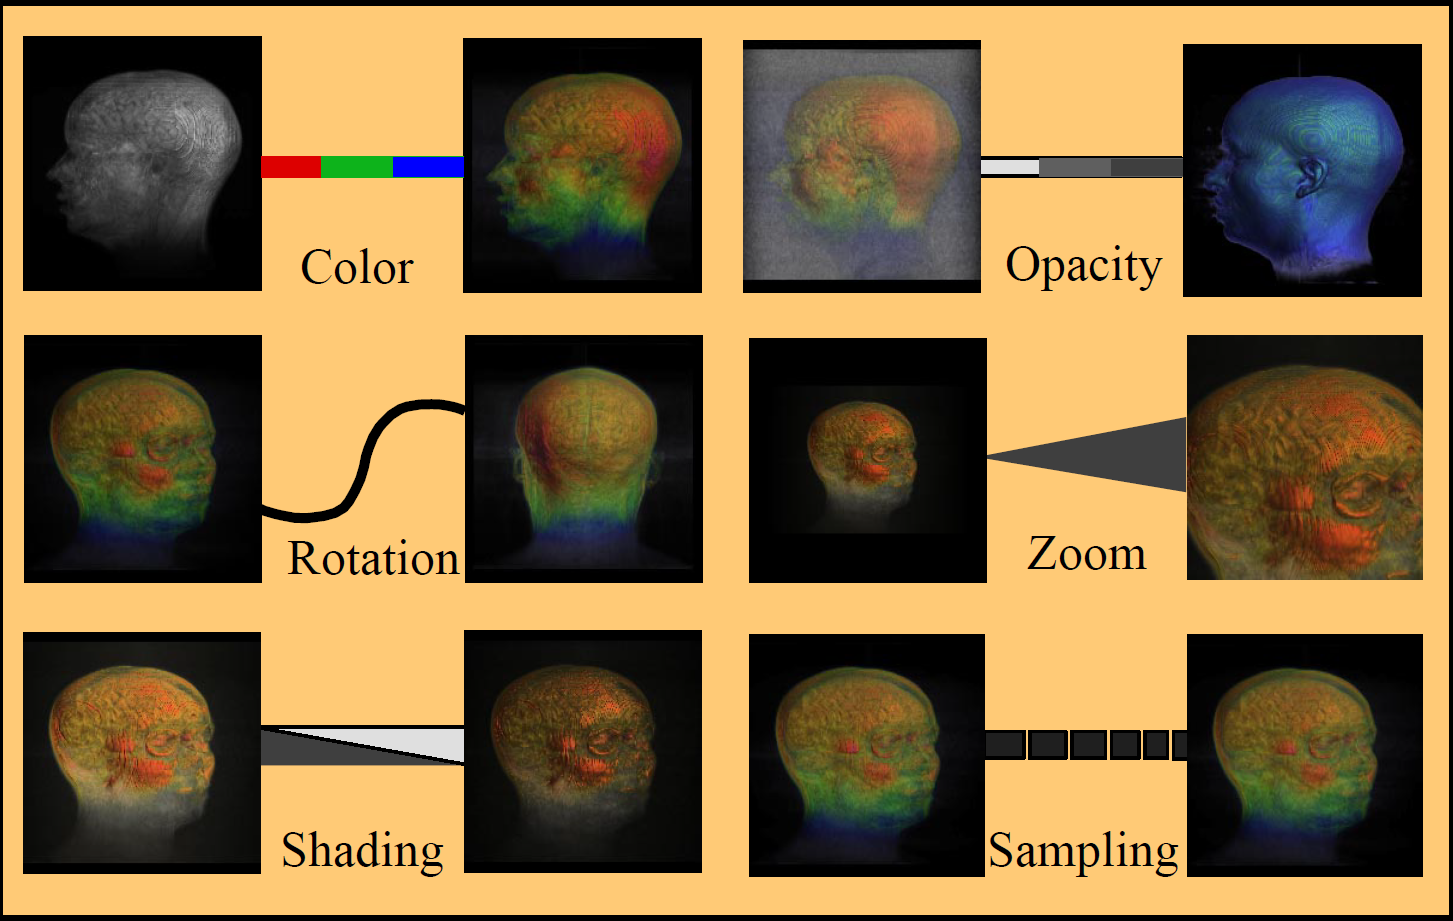
\includegraphics[width=.7\columnwidth]{action-2}}
\caption{Visual representations of actions.}
\end{figure}

timeline: manual 

\subsubsection{Interaction}

\subsection{Tree}
Overview of using tree/graph to visualize branching history

\begin{figure}[!htb]
	\centering
	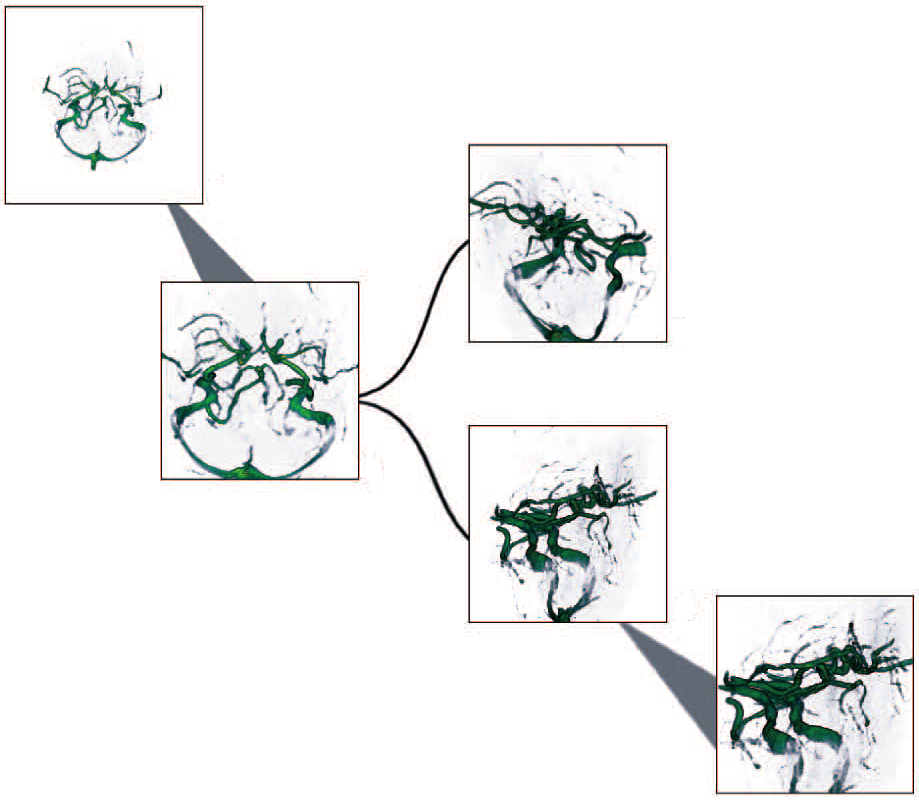
\includegraphics[width=.7\columnwidth]{tree}
	\caption{Tree visualization of branching history. \emph{Source:~\cite{Jankun-Kelly2007}}.}
	\label{fig:lr-tree}
\end{figure}

Techniques to handle large graph

Encode time into the graph nodes

%\paragraph{Layout of Actions and States}
%Typically, the system begins with an initial state (node). When the user performs an action, a new node is created for the current state, and a new edge is added to connect the previous node with the current node. Gradually, a string of nodes and edges is built in the chronological order. The system can support revisiting to the previous state. If a new action is performed at that state, a new branch will be forked to store forthcoming actions. Therefore, the analysis process has the layout of a \textit{direct acyclic graph}, or a \textit{tree} if revisited links are not explicitly visualized.

%To not distract analysts from the primary data exploration and save space, several techniques have been proposed to reduce the display area of the provenance graph: organising trees in the right horizontal-vertical layout \cite{Shrinivasan2008}, displaying only nodes of the active branch that led to the selected visualization \cite{Klemmer2002}, allowing graph nodes be expandable/collapsible on demand \cite{Bavoil2005}, supporting zoom-able and pan-able interface \cite{Dunne2012}, and applying distortion techniques to focus on more relevant states \cite{Meng1998}.

%The order of actions can be interpreted through the direction of edges in the provenance graph. Moreover, exact time gap between actions can also be measured and visually encoded into the visualization. VisTrails \cite{Bavoil2005} colour-codes the background of visualization nodes according to when they are created (Figure \ref{fig:lr-tree-time-1}); and Aruvi \cite{Shrinivasan2008} uses the length of edges to represent the distance in terms of time between two states (Figure \ref{fig:lr-tree-time-2}). This time indication can be updated only when a new node is added, or continuously to reflect the fact that time is always flying. In the latter case, endlessly, background nodes will become lighter and edge lengths will become shorter. This \textit{time-travel} interface is implemented in Visage \cite{Derthick2001}. %TODO: Kai: it's not clear

Focus and context

\begin{figure}[!htb]
\centering
\subcaptionbox{Node backgrounds are color coded based on time. \emph{Image source:~\cite{Bavoil2005}}.\label{fig:lr-tree-time-1}}[.3\columnwidth]{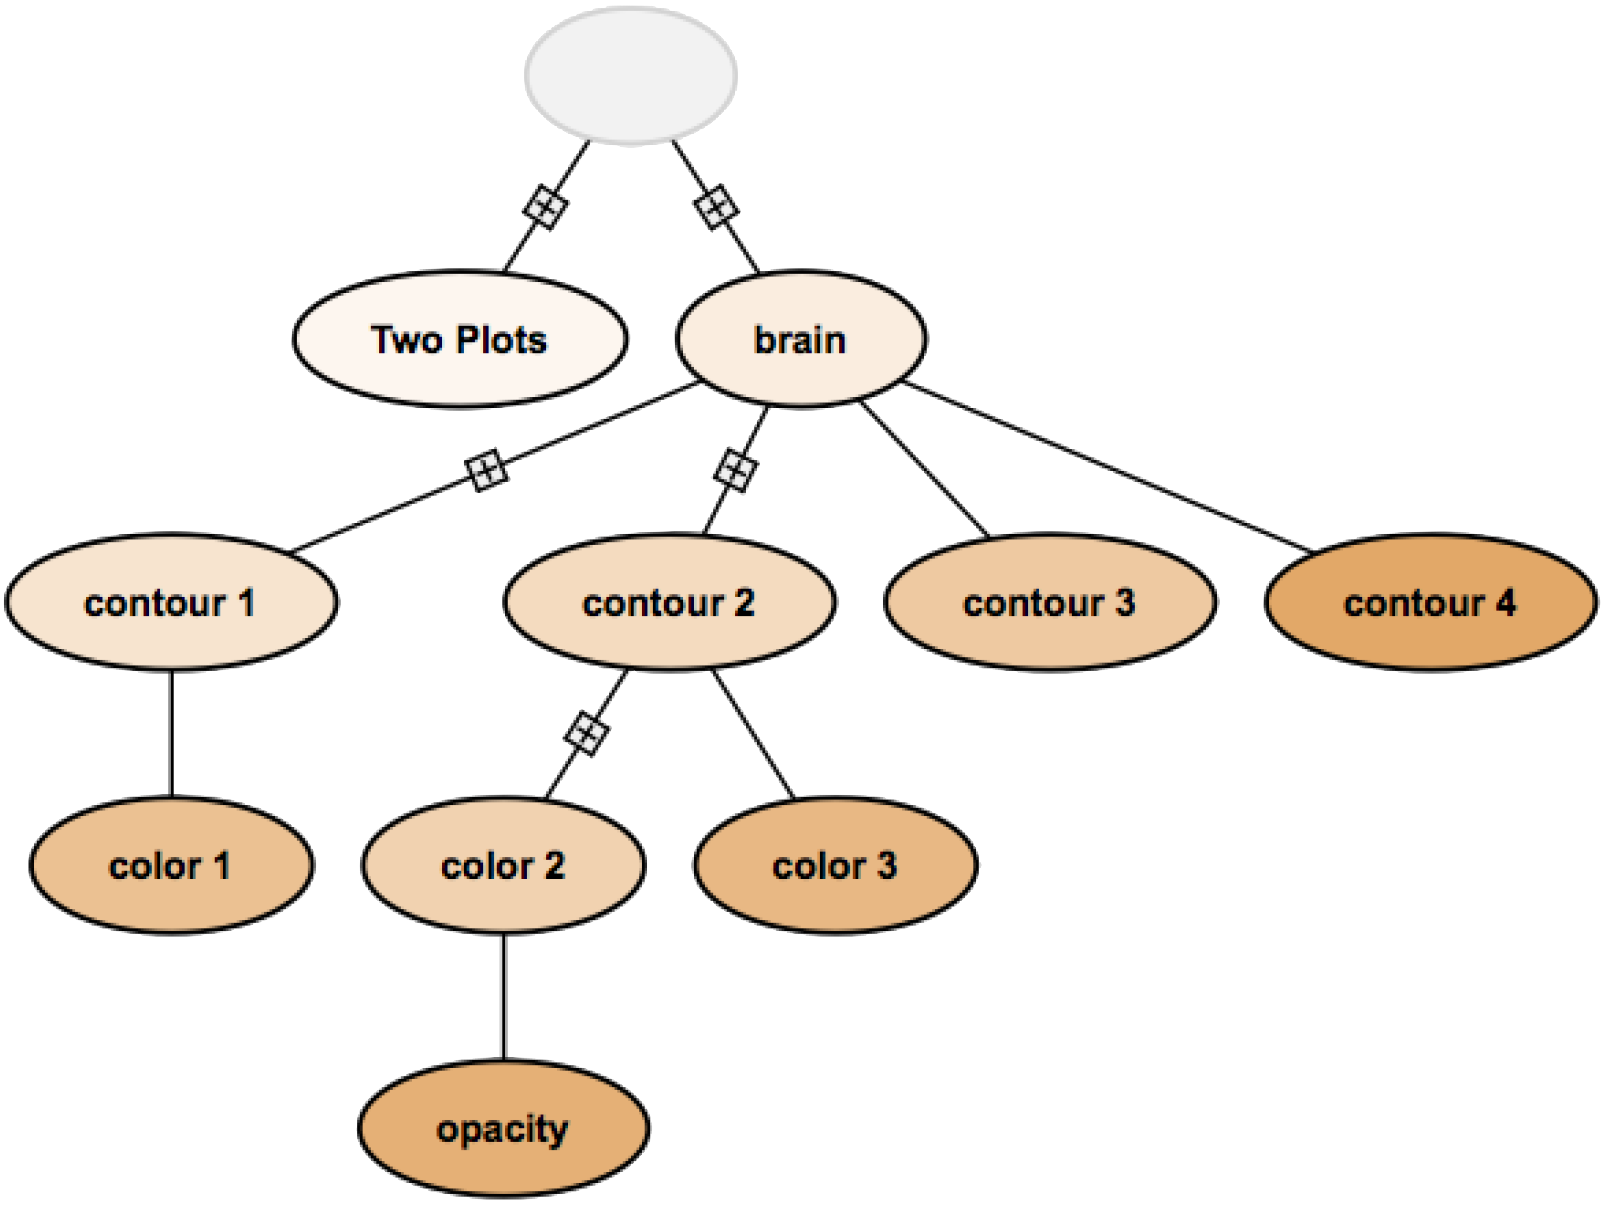
\includegraphics[height=0.21\columnwidth]{tree-time-1}} 
\hfill
\subcaptionbox{The edge length between two nodes represents the interval between them. \emph{Image source:~\cite{Shrinivasan2008}}.\label{fig:lr-tree-time-2}}{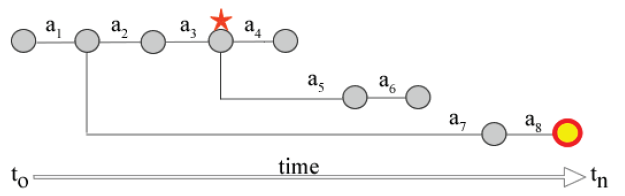
\includegraphics[height=0.21\columnwidth]{tree-time-2}}
\caption{Encoding temporal information into provenance graphs.}
\end{figure}

%The provenance space can be unified with the data exploration space, where each node of the provenance graph represents a fully interactive visualization. Zoom-able and pan-able interface needs to be supported to allow users either to focus on the current visualization  (Figure \ref{fig:focus}) or to observe the entire context of the analysis process (Figure \ref{fig:context}).

\begin{figure}[ht]
\centering
\subcaptionbox{Focus view on the active visualization.}{\label{fig:focus}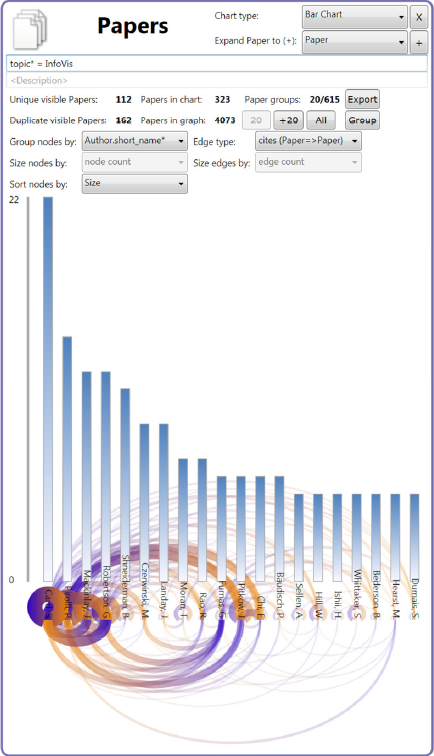
\includegraphics[height=0.57\columnwidth]{GraphTrail-Focus.png}} \hspace{0.1cm}
\subcaptionbox{Context view to see the overview of what has been done.}{\label{fig:context}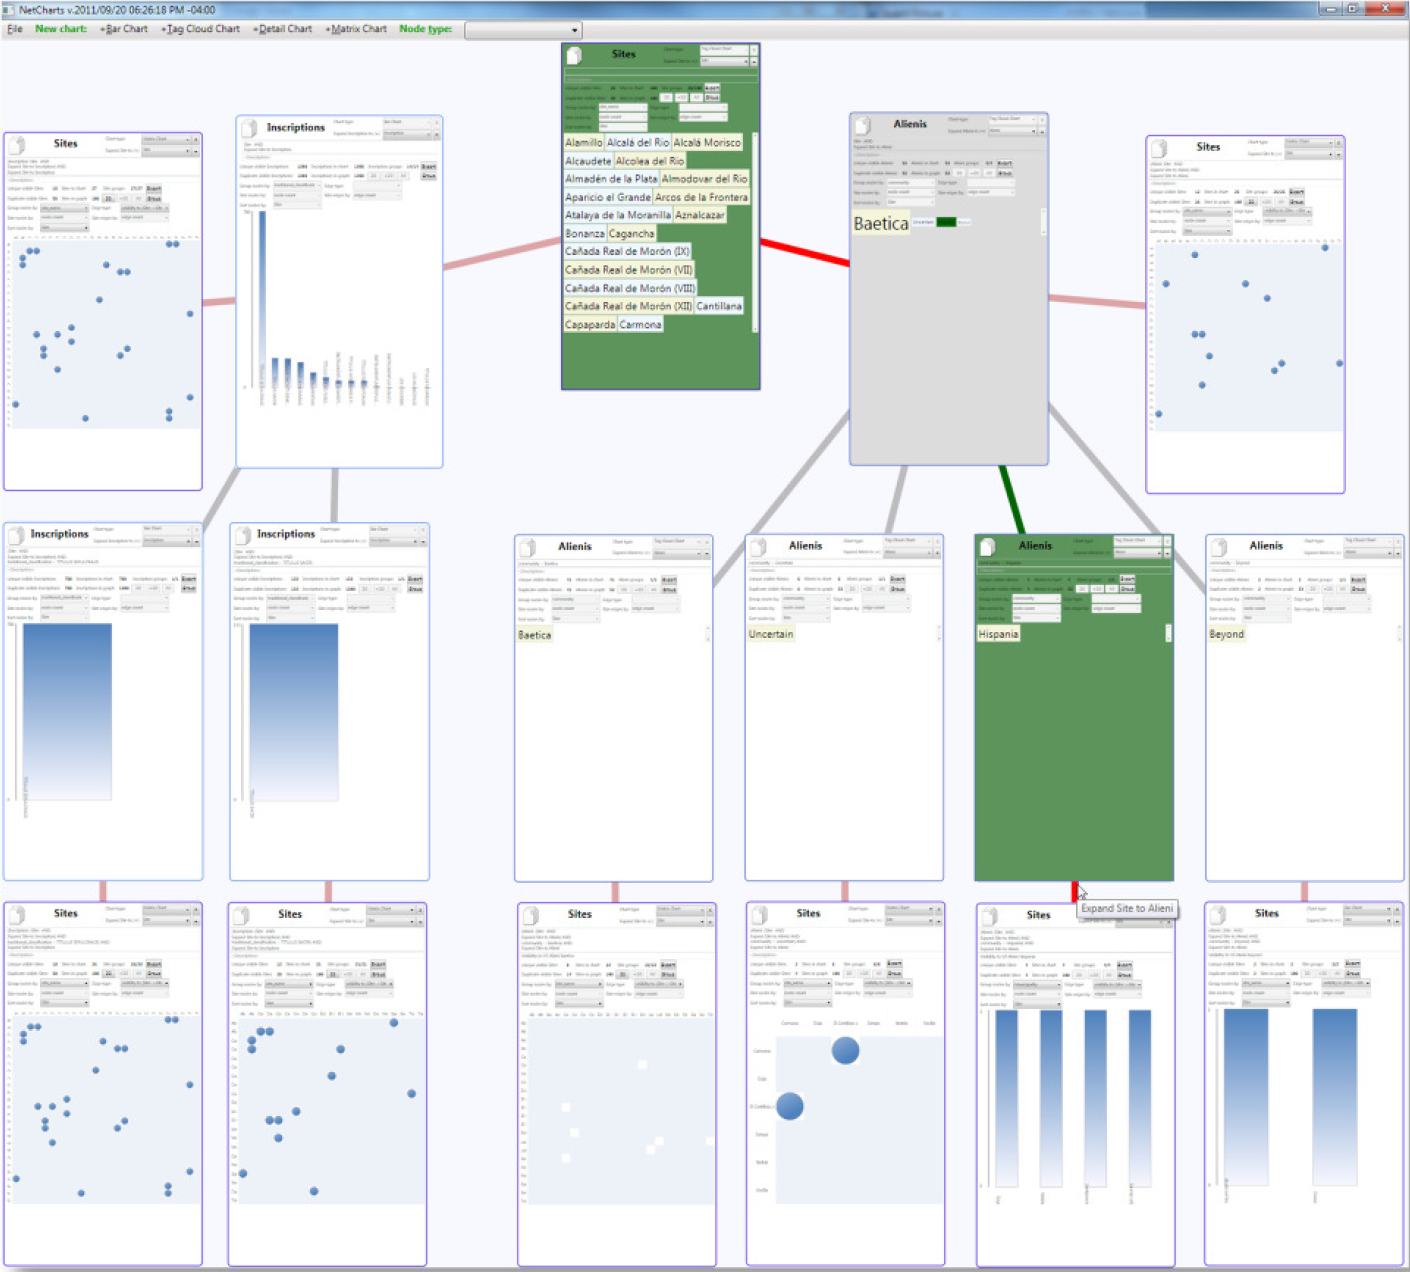
\includegraphics[height=0.57\columnwidth]{GraphTrail-Context.png}}
\caption{Integration of the provenance graph into the data exploration space. \emph{Image source:~\cite{Dunne2012}}.}
\label{fig:IntegratedView}
\end{figure}

\subsubsection{Visualizing the Reasoning Process}
\label{sub:reasoningprocess}
The Aruvi system \cite{Shrinivasan2008} allows analysts to freely compose the reasoning process by using a graphical editor. Users can take note in rectangles or ellipses, and use arrows to connect them. Conventionally, nodes can be referred as \textit{evidence}, \textit{assumptions} or \textit{hypotheses}, and arrows can be referred as \textit{causal relationships}. Nodes in the editor can be linked to the captured visualizations to help explain its reasoning, and these nodes are marked with a star to indicate the existence of the linked visualizations. Instead of using a graphical editor and an implicit convention to map drawing shapes with reasoning artefacts, Scalable Reasoning System \cite{Pike2009a} provides a more formal method to document the reasoning process. A captured visualization can be dropped to the reasoning space to create a node. The node shows the miniature of the captured visualization and can be tagged as an \textit{evidence} artefact. An evidence can be converted to a \textit{casual relationship} and its rectangular shape will become an edge. An \textit{assumption} is a free note and can be upgraded as a \textit{hypothesis} when it is supported by an evidence. Figure \ref{fig:ReasoningDocumenting} shows those two examples of reasoning process visualization.

\begin{figure}[ht]
\centering
\subcaptionbox{Using graphical editor to freely construct the mental model \cite{Shrinivasan2008}.}{\label{fig:knowledgeview}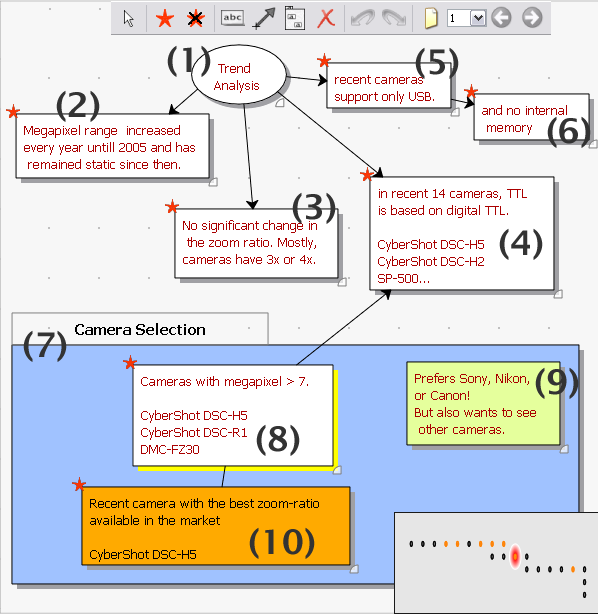
\includegraphics[height=0.39\columnwidth]{Knowledge-View.png}} \hspace{0.1cm}
\subcaptionbox{A formal reasoning diagram with different types of artefacts: evidence, casual relationship, assumption and hypothesis \cite{Pike2009a}.}{\label{fig:reasoningworkspace}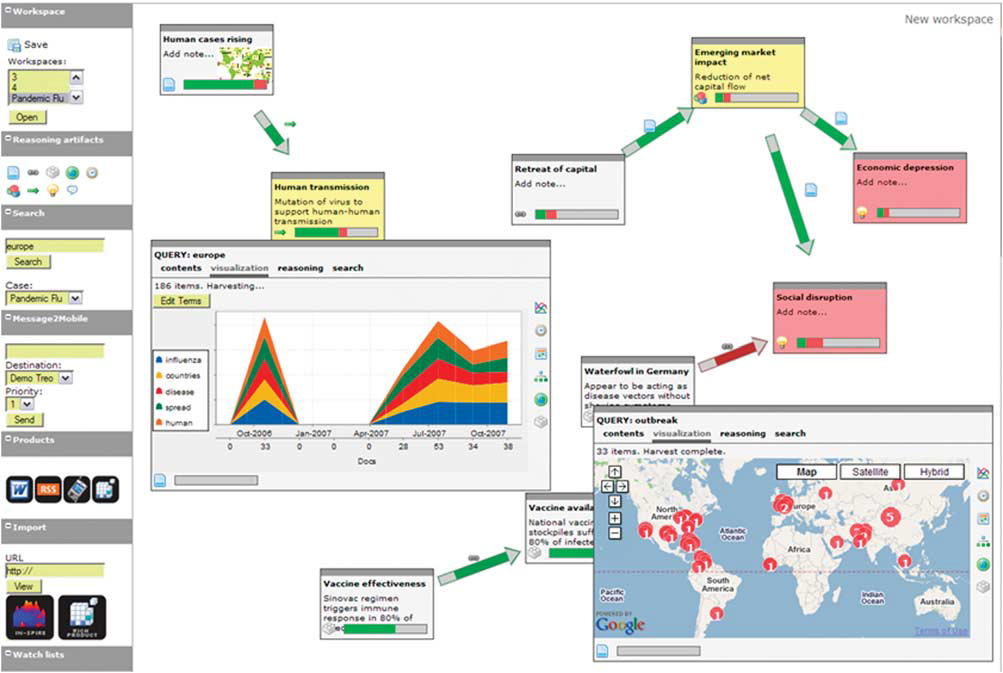
\includegraphics[height=.39\columnwidth]{Reasoning-Workspace.png}}
\caption{Examples of visualizing the reasoning process.}
\label{fig:ReasoningDocumenting}
\end{figure}

%\begin{figure}[ht]
%\centering
%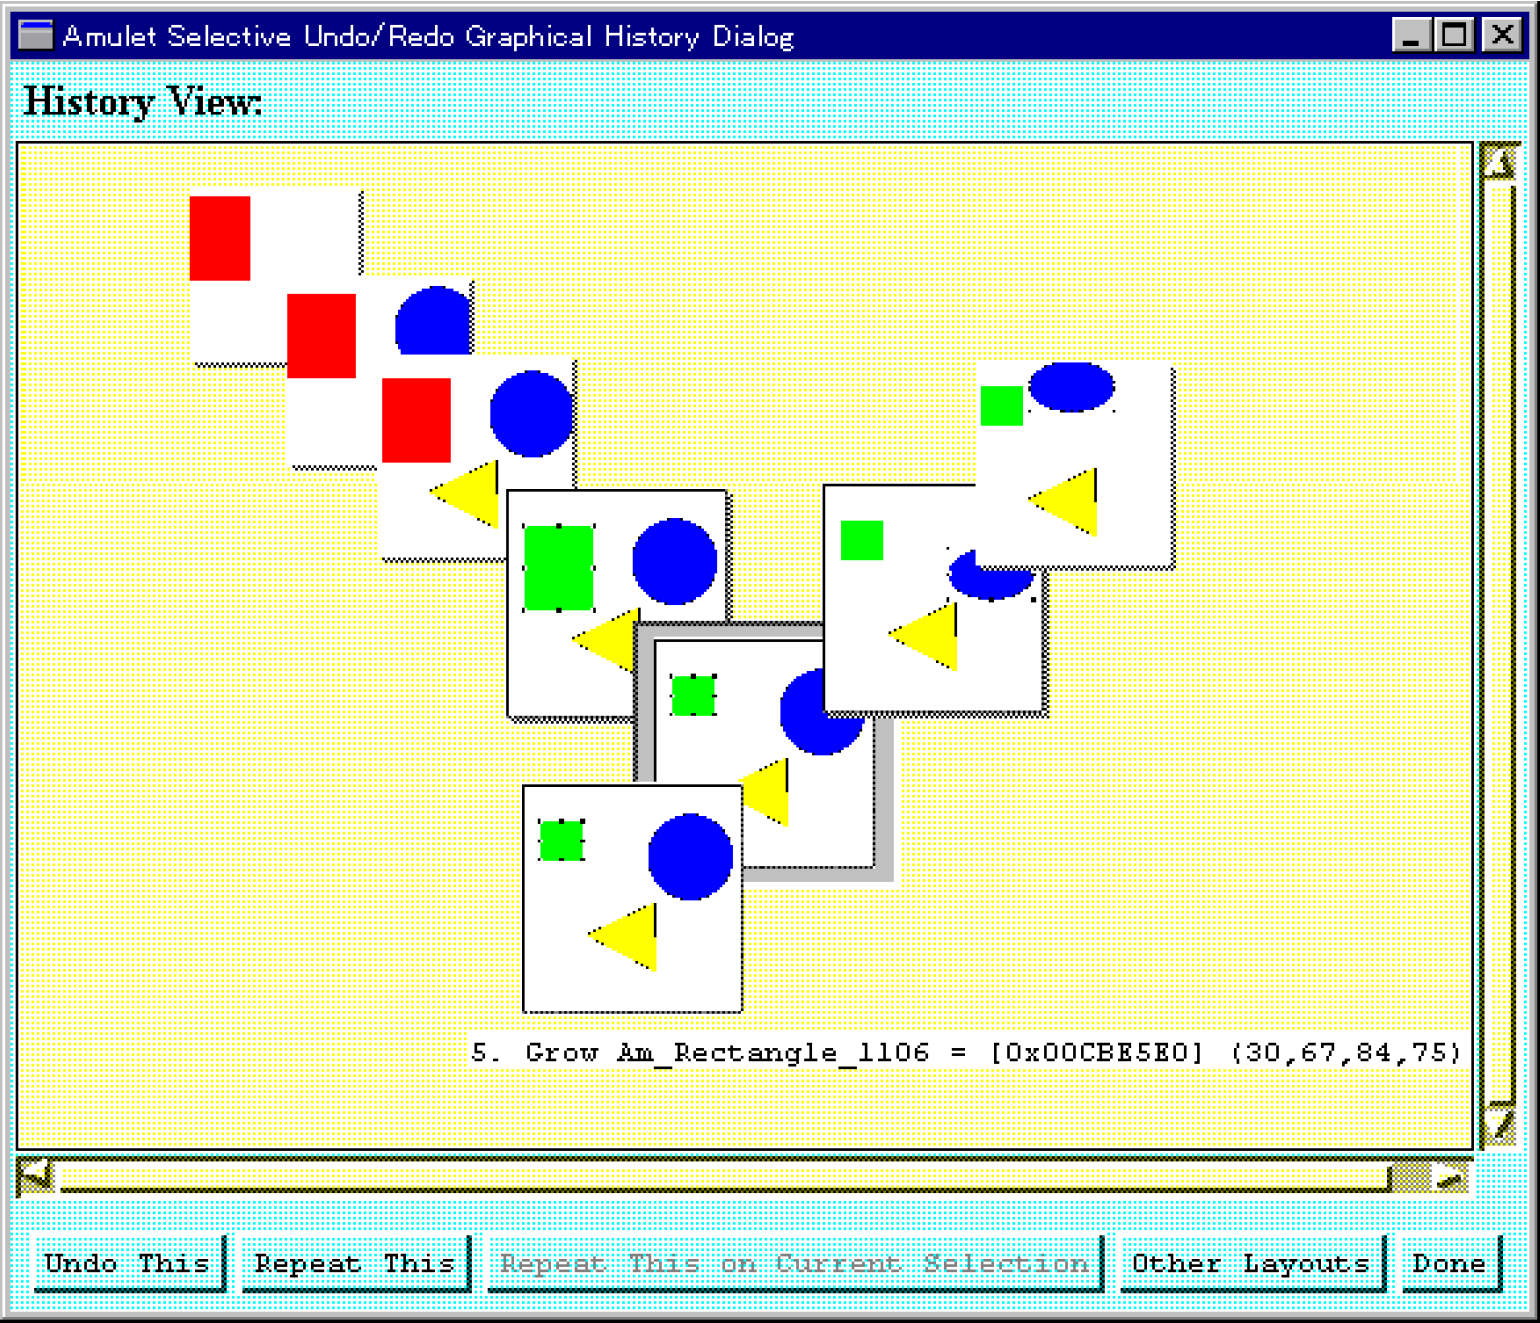
\includegraphics[width=.7\textwidth]{Perspective-View.png}
%\caption{An example of using perspective view in provenance visualization layout: further objects are smaller \cite{Meng1998}.}
%\label{fig:Perspective-View}
%\end{figure}

%\subsubsection{Other Techniques}
%Instead of displaying the history of actions in a temporal order, other factors can be used to reveal different aspects of the analysis process; for example, the flow of data retrieved during the course of the analysis is shown in the \textit{dependency graph} \cite{Kadivar2009} (Figure \ref{fig:Dependency-Graph}). The implemented system uses a scripting language to model the analysis process and each set of retrieved data is assigned to a variable; and thus, uses variable names to visualize the active data in each analysis step. However, this method may not be easy to apply to a generic non-scripting language system because it is not easy to visualize the difference between each set of data.
%
%\begin{figure}[ht]
%\centering
%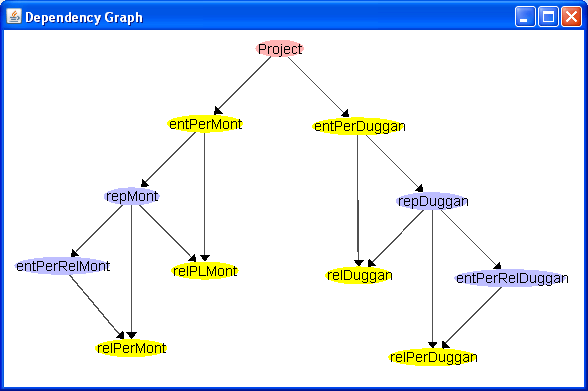
\includegraphics[width=.75\textwidth]{Dependency-Graph.png}
%\caption{Dependency graph of the analysis session of a scenario from the novel \textit{The Day of the Jackal} \cite{Kadivar2009}. First, the analyst searches for person \textit{Montpellier} and the result is assigned to \textit{entPerMont}. Then, all reports related to Montepellier are fetched to \textit{repMont}. All persons mentioned in those reports are listed for further investigation (\textit{entPerRelMont}). The analyst notices on \textit{Duggan} and continues investigating that person. This is the flow that the analyst investigates the case; however, in the data perspective, after noticing Duggan, the analyst restarts the steps as he or she did with Montepellier. Therefore, in terms of data, Montepellier and Duggan are two independent branches in the data analysis tree.}
%\label{fig:Dependency-Graph}
%\end{figure}
%
%Another method to recall the analysis process is through the statistical usages of the system such as the most used visualization tools and most investigated data objects \cite{Shrinivasan2009a}. This method provides a good overview of the analysis; however, it cannot show the sequence of actions performed during the analysis.
